\section{\nn{} Runtime Energy Adaptation} \label{sec:method2}

\nn{} runtime energy adaptation utilises the presented runtime energy profiling to dynamically adapts the voltage threshold to the latest energy consumption of a task. 
This method assumes the system is able to monitor the supply voltage and signal the MCU to wake up or sleep when a high or low threshold is hit, and the threshold is configurable by the MCU at runtime. 
The voltage monitoring ability is widely required by prior IPSs in the forms of a voltage comparator~\cite{kang2018homerun, balsamo2016hibernus++}, an energy management unit~\cite{gomez2016dynamic, maeng2019supporting}, or a periodic ADC polling~\cite{sliper2019efficient}. 

\nn{} runtime energy adaptation is decoupled with the method of energy profiling. 
The adaptation scheme requires an interface of the energy profiling method that can return a profiling result and trigger an instance of profiling.

The fundamental goal of runtime energy adaptation is to allocate a barely sufficient energy budget for each task. 
Its routine is also expected to have as little overheads as possible, run energy profiling as infrequently as possible, while react to energy variations as quickly as possible.


% Outline
% goal
% basic adaptation for constant operation
%   flowchart
% optional linear adaptation
% optional multiple configurations (can be similar to multiple atom_func_state)

Goal: Reduce unnecessary/redundant measurements and take necessary measurements.

Enable voltage threshold adaptation against runtime variation of energy consumption due to unforeseeable operating conditions, and also enable linear adaptation to function knobs that are known to the system. 

\begin{itemize}
    \item Without function knobs: use the latest profiled threshold.
    \item With function knobs: do a linear regression based on a number of recent measurements. 
\end{itemize}


With a target end voltage $\symb{V}{end}$ below which the system fails, the voltage threshold $\symb{V}{th}$ that the system should set to ensure a task's completion is
\begin{equation}
    \symb{V}{th} = \symb{V}{end} + \Delta \symb{V}{task}
\end{equation}

\subsection{Adaptation Routine}

\begin{figure}
    \centering
    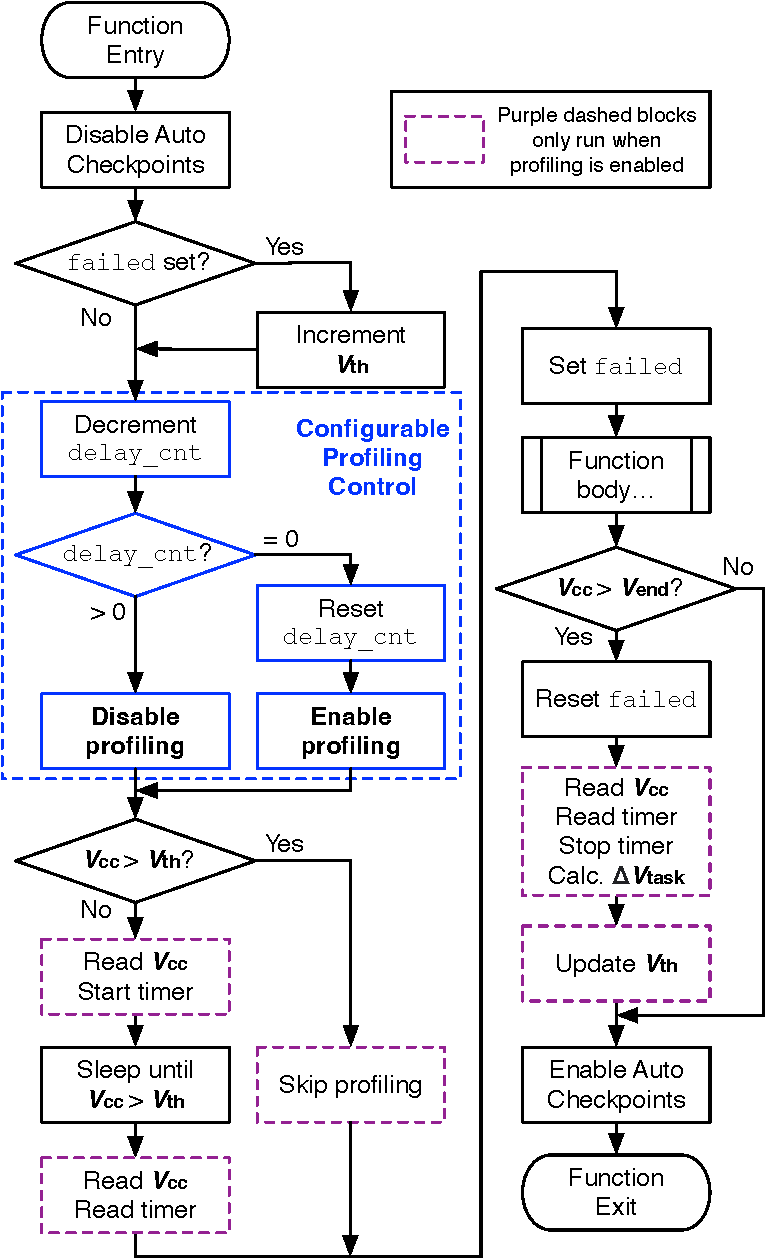
\includegraphics[width=0.8\columnwidth]{ch5_optic/figures/flowchart.pdf}
    \caption{Flowchart of \nn{}'s runtime energy adaptation scheme. The dashed blue blocks represent a configurable control logic to decide when to perform energy profiling. The dashed purple blocks represent the energy profiling routine which is only run when the profiling is triggered. The solid purple block is where \nm{V}{th} is updated with the newly profiled result and is also only run when the profiling is triggered. }
    \label{fig:opta_flowchart}
\end{figure}

\subsection{Linear Adaptation}

\subsection{Discussion}

The ability to fall back differentiates it from a "simply-incrementing-threshold" DEBS.
